\documentclass{report}


\usepackage{graphicx}

\usepackage{amsmath}
\usepackage{graphicx}
\usepackage{ulem}
\usepackage{float}
\usepackage[utf8]{inputenc}
\usepackage{gensymb}
\usepackage{amsmath}
\usepackage{amssymb}
\usepackage{mathtools}
\newcommand{\partder}[1]{\frac{\partial h^l}{\partial #1}}

\graphicspath{{figures/}}

\title{OCS Hints for Questions}
\author{Julian Wolf}
\begin{document}
\maketitle
%%%%%%%%%%%%%%%%%%%%%%%%%%%%%%%%%%%%%%%%%%%%%%%%%%%%%%%%%%%%%%%%%%
\section*{Derivations}
Die Antworten sind teilweise unvollständig, einerseits, weil er die Antworten als "Eh Klar" abgestempelt hat, anderer seits weil er so schnell durchging, dass ein Mitschreiben nicht mehr möglich war. 

\begin{enumerate}
%%%%%%%%%%%%%%%%%%%%%%%%%%%%%%%%%%%%%%%%%%%%%%%%%%%%%%%%%%%
\item Draw level lines and arrows
\begin{itemize}
\item objective function is the function we want to minimize
\item constraint set is a set of functions
\item optimal solution: find $f(x^*) \leq f(x), \forall x \in X$
\item level set: compareable to level lines of terrain, convex function $=>$ convex level set (but there are non convex fct with convex level sets), 
\end{itemize}

%%%%%%%%%%%%%%%%%%%%%%%%%%%%%%%%%%%%%%%%%%%%%%%%%%%%%%%%%%%
\item 
\begin{itemize}
\item \textbf{Linear}: Objective Function and Constraints may only be linear
$min\ c^Tx, s.t.\ Ax \leq b, x \geq 0$\\
Polynomial solvable
\item \textbf{Non Linear}: Objective Function and Constriants may  be non linear
$min\ \frac{1}{2} x^TQx + c^Tx, s.t.\ Ax \leq b, Ex = d$\\
Q symmetrical and pos. definite, polynomial solvable
\item \textbf{Quadratic}: objective function is quadratic, constraints are linear	
$min_{x \in \mathbb{R}}\ f_0(x) \texttt{ (objective)},$\\
$s.t.\ f_i(x) \leq i=0..m \texttt{ (contraints)}$\\
polynomial time
\item \textbf{convex set}: 
$\alpha x + (1 - \alpha)y \ in X, \forall x, y \in X, \alpha \in [0, 1]$
\item \textbf{convex fct}:
$f(\alpha x + (1 - \alpha)y) \leq \alpha f(x) + (1 - \alpha)f(y) , \forall x, y \in X, \alpha \in [0, 1]$ 
\end{itemize}
%%%%%%%%%%%%%%%%%%%%%%%%%%%%%%%%%%%%%%%%%%%%%%%%%%%%%%%%%%%
\item 
\begin{itemize}
	\item When hessian is strictly positive, it is a strict global maximum
	\item \textbf{unconst Local minimum:} $f(x^*) \leq f(x), \forall x \texttt{ with } || x - x^* || \leq \varepsilon$
	\item \textbf{unconst global minimum:} $f(x^*) \leq f(x), \forall x \in \mathbb{R}$
\end{itemize}

\begin{figure}[H]
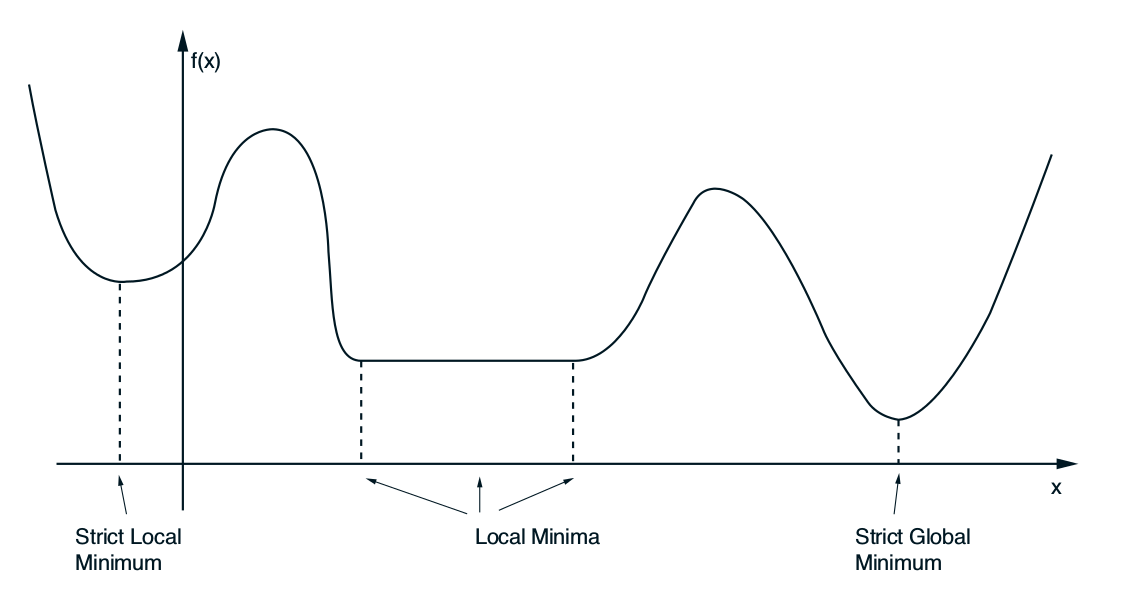
\includegraphics[scale=0.3]{loc_glob_min.png}
\caption{Local/Global minimas\label{fig:min}}
\end{figure}	
%%%%%%%%%%%%%%%%%%%%%%%%%%%%%%%%%%%%%%%%%%%%%%%%%%%%%%%%%%%
\item If positive and negative Eigenvalues, we can not define convexity
%%%%%%%%%%%%%%%%%%%%%%%%%%%%%%%%%%%%%%%%%%%%%%%%%%%%%%%%%%%
\item 
\begin{itemize}
\item Descent direction: angle of step and derivation direction $< 90^\circ$
\end{itemize}

%%%%%%%%%%%%%%%%%%%%%%%%%%%%%%%%%%%%%%%%%%%%%%%%%%%%%%%%%%%
\item Identity, Hessian, Gauss Newton, Diag Hessian, zik zak
%%%%%%%%%%%%%%%%%%%%%%%%%%%%%%%%%%%%%%%%%%%%%%%%%%%%%%%%%%%
\item upper bound, \sout{... too fast...}
%%%%%%%%%%%%%%%%%%%%%%%%%%%%%%%%%%%%%%%%%%%%%%%%%%%%%%%%%%%
\item Energy convergence 
%%%%%%%%%%%%%%%%%%%%%%%%%%%%%%%%%%%%%%%%%%%%%%%%%%%%%%%%%%%
\item \sout{too fast}
%%%%%%%%%%%%%%%%%%%%%%%%%%%%%%%%%%%%%%%%%%%%%%%%%%%%%%%%%%%
\item \sout{polynomial euqations, distance to std. Newton}
%%%%%%%%%%%%%%%%%%%%%%%%%%%%%%%%%%%%%%%%%%%%%%%%%%%%%%%%%%%
\item incremental of gauss newton
%%%%%%%%%%%%%%%%%%%%%%%%%%%%%%%%%%%%%%%%%%%%%%%%%%%%%%%%%%%
\item \sout{too fast}
%%%%%%%%%%%%%%%%%%%%%%%%%%%%%%%%%%%%%%%%%%%%%%%%%%%%%%%%%%%
\item \sout{iterative}
%%%%%%%%%%%%%%%%%%%%%%%%%%%%%%%%%%%%%%%%%%%%%%%%%%%%%%%%%%%
\item nesterov in gradient, heavy-ball just in point
%%%%%%%%%%%%%%%%%%%%%%%%%%%%%%%%%%%%%%%%%%%%%%%%%%%%%%%%%%%
\item in subspace reduce to eq, what is a subspace?
%%%%%%%%%%%%%%%%%%%%%%%%%%%%%%%%%%%%%%%%%%%%%%%%%%%%%%%%%%%
\item First pages of slide 10
%%%%%%%%%%%%%%%%%%%%%%%%%%%%%%%%%%%%%%%%%%%%%%%%%%%%%%%%%%%
\item middle/end of pages slide 10 - start in interior and just take small steps $->$ we can ignore constraint under these conditions
%%%%%%%%%%%%%%%%%%%%%%%%%%%%%%%%%%%%%%%%%%%%%%%%%%%%%%%%%%%
\item \sout{too fast}
%%%%%%%%%%%%%%%%%%%%%%%%%%%%%%%%%%%%%%%%%%%%%%%%%%%%%%%%%%%
\item see figure~\ref{fig:ex1}

%%%%%%%%%%%%%%%%%%%%%%%%%%%%%%%%%%%%%%%%%%%%%%%%%%%%%%%%%%%
\item see figure~\ref{fig:ex2}

%%%%%%%%%%%%%%%%%%%%%%%%%%%%%%%%%%%%%%%%%%%%%%%%%%%%%%%%%%%
\item see figure~\ref{fig:ex2}


\end{enumerate}
\begin{figure}[H]
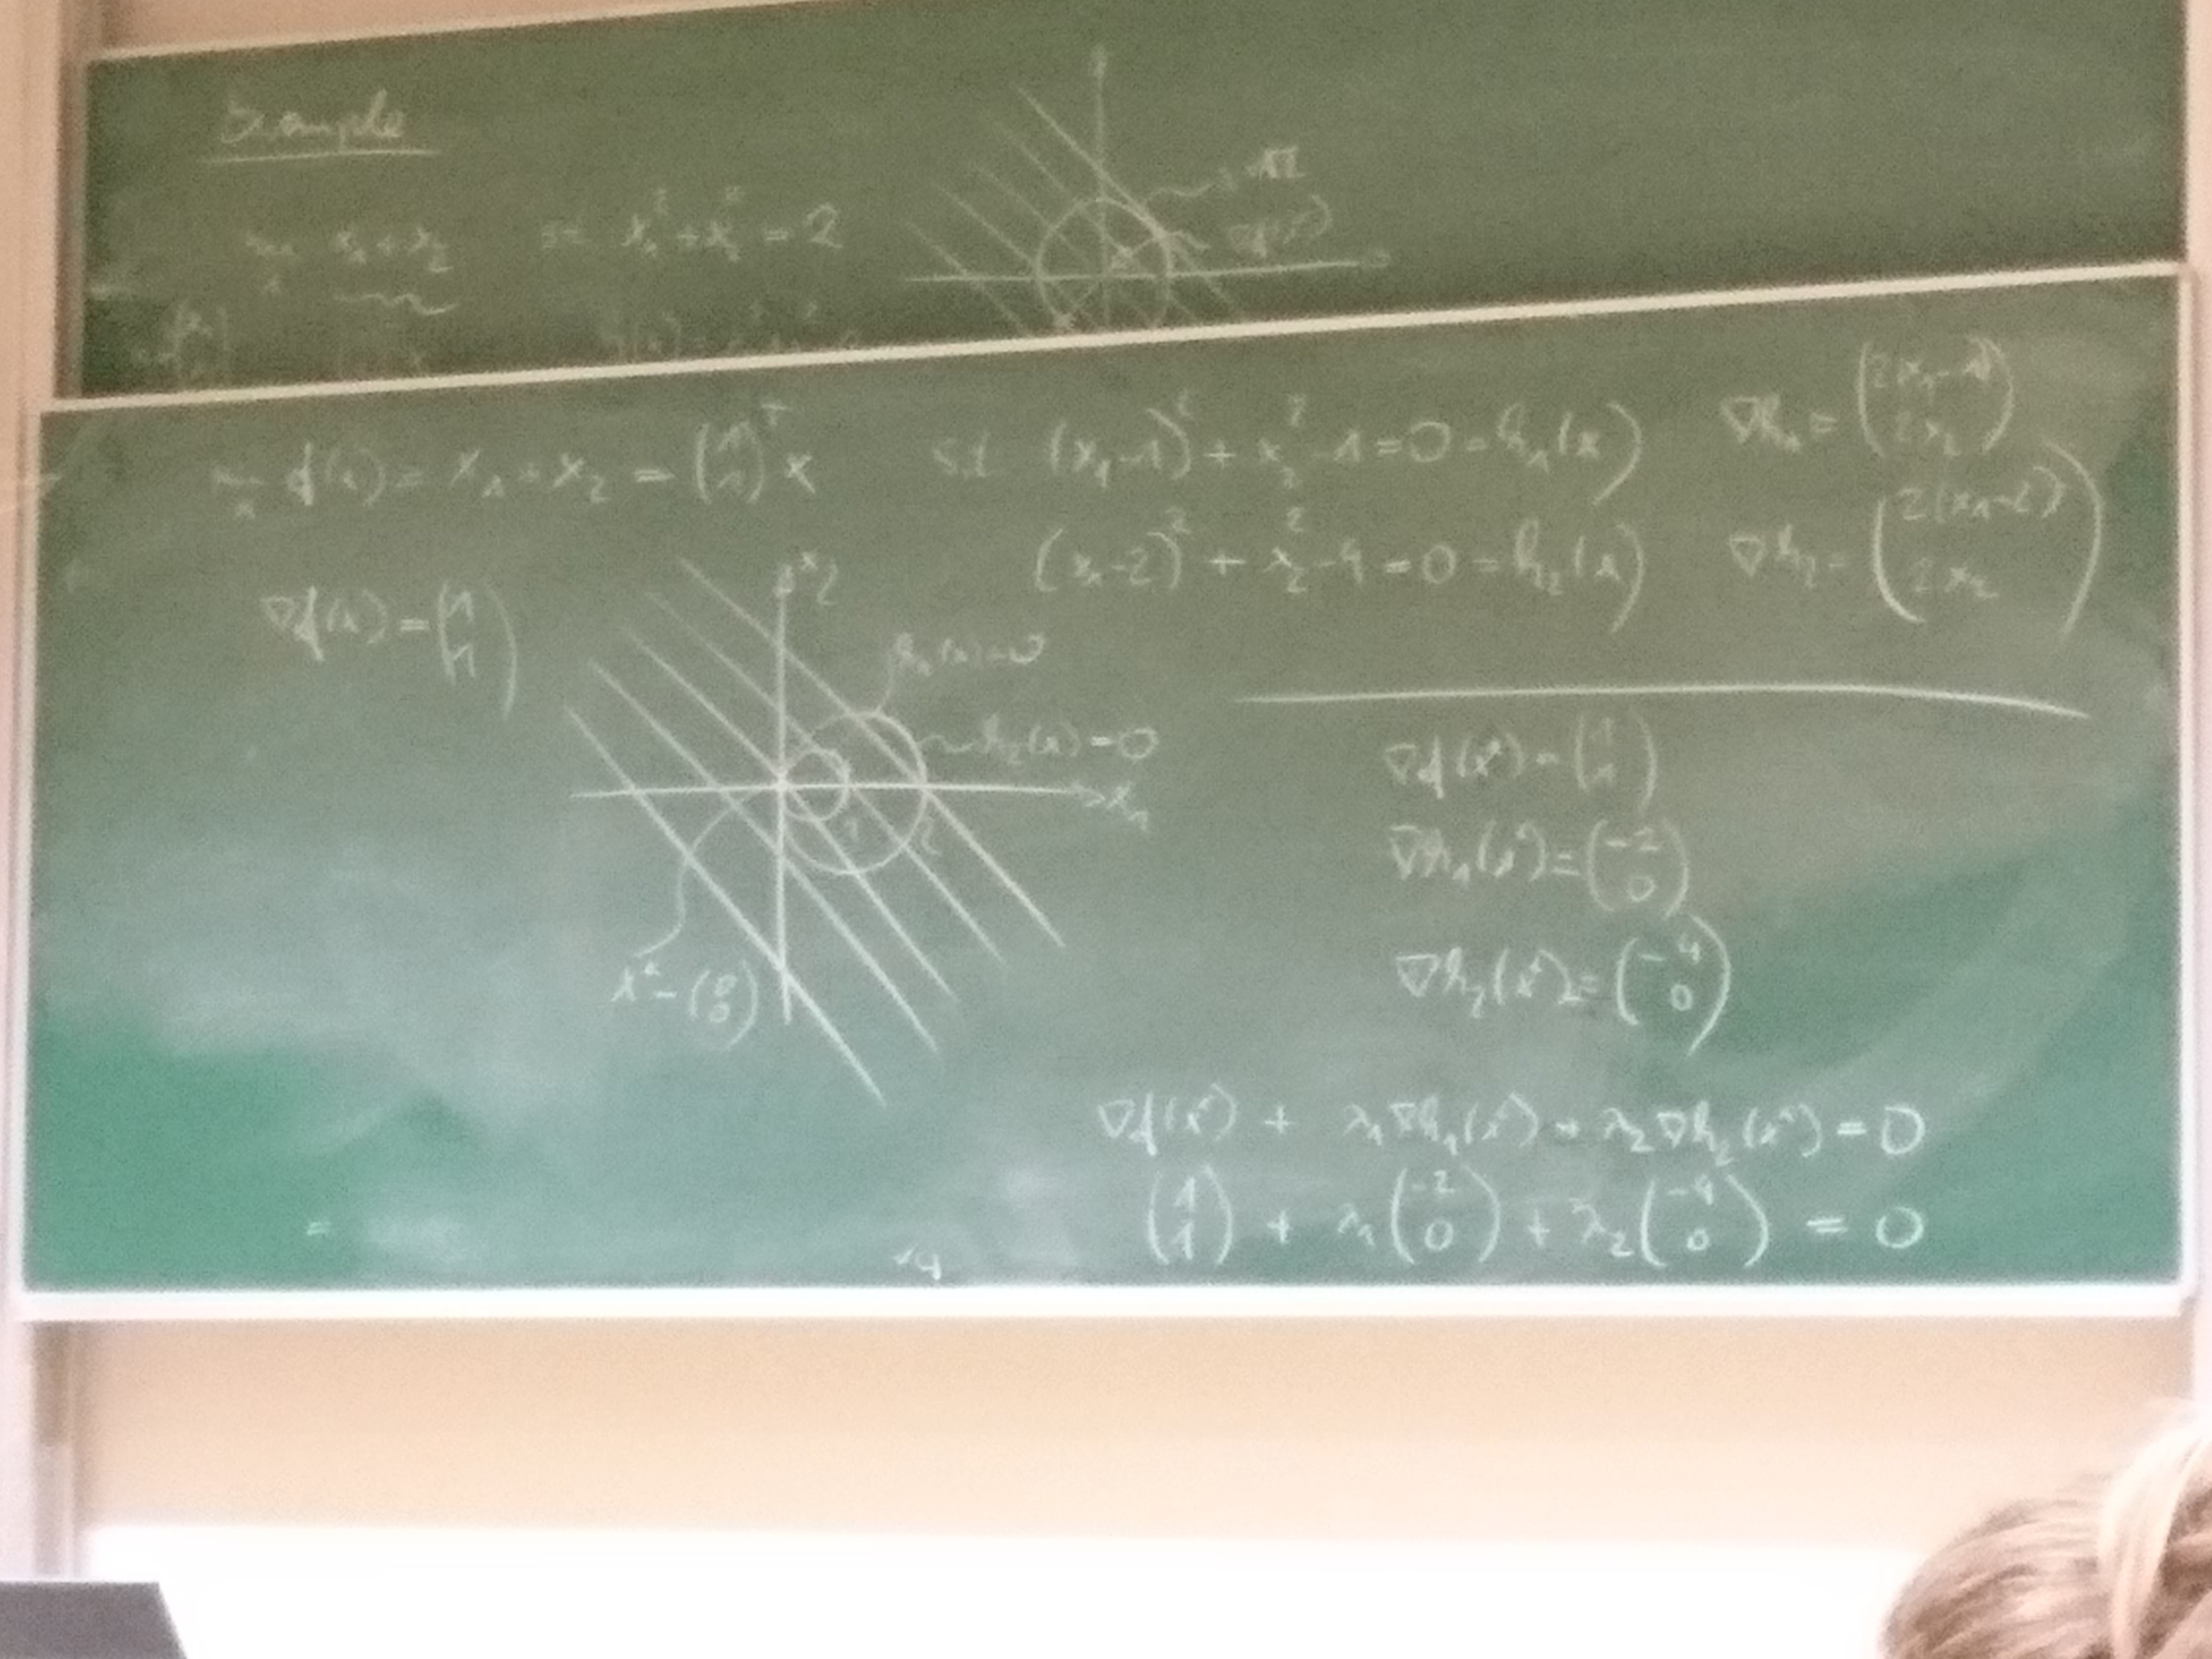
\includegraphics[scale=0.08]{2017_01_24-ex1.jpg}
\caption{Example1,  24.01.2017\label{fig:ex1}}
\end{figure}

\begin{figure}[H]
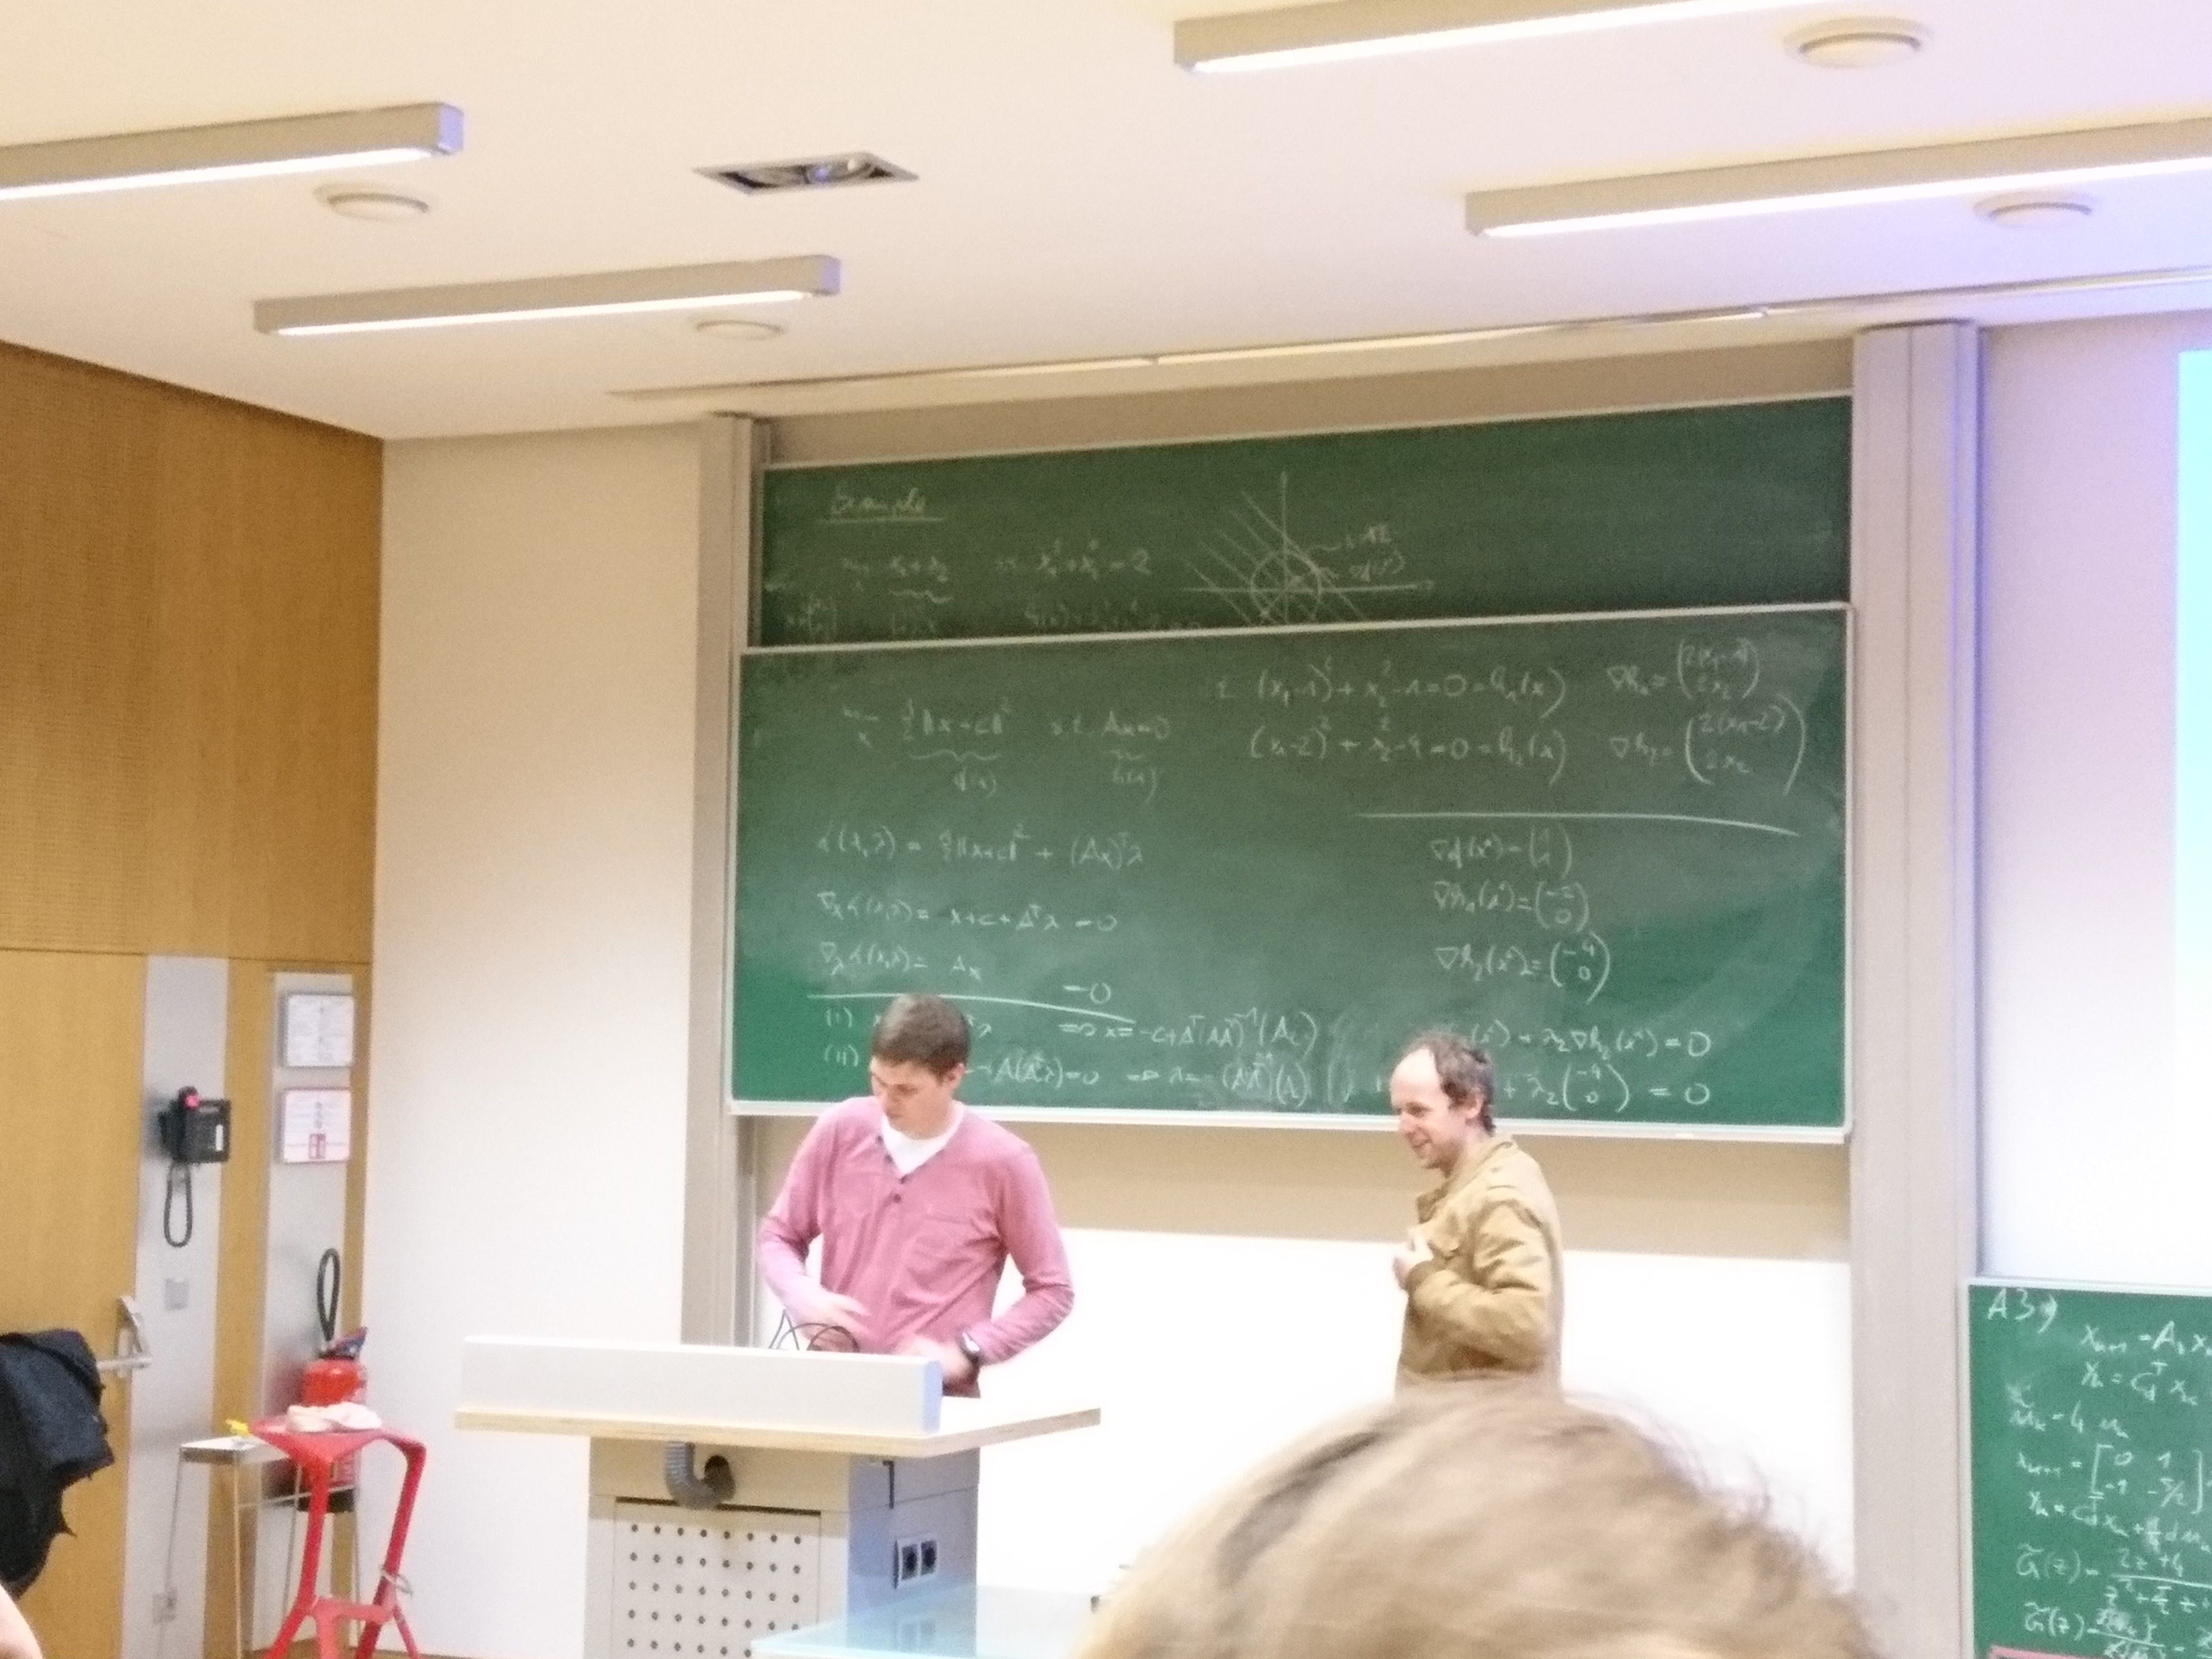
\includegraphics[scale=0.08]{2017_01_24-ex2.jpg}
\caption{Example 2,  24.01.2017\label{fig:ex2}}
\end{figure}
\end{document}
